\chapter{Funktionen} 

Jedem von euch sollte in der Zwischenzeit bewusst geworden sein, dass es in der Mathematik sehr viel um
Gleichungen geht. Der Begriff der Gleichung ist und wird auch f\"{u}r die n\"{a}chsten Jahre (zumindest im
Mathematikunterricht) ein zentraler Begriff bleiben. Neben dem Begriff der Gleichung existiert ein weiterer
sehr wichtiger Begriff und  zwar die Funktionen.

In diesem Abschnitt gibt es die erste Einf�hrung;  wichtig ist nun sich mit diesem Kapitel sehr gut vertraut
zu machen, denn die enorme Bedeutung kann hier gar nicht zum Ausdruck gebracht werden.


\subsection*{Wozu sind Funktionen gut?}





Immer dann, wenn der Wert einer Gr��e vom Wert einer anderen Gr��e {\it abh�ngt}, liegt eine Funktion vor. Da die Natur und unser Leben voll von solchen Abh�ngigkeiten sind, kann eine unermesslich gro�e Anzahl von Vorg�ngen und Zusammenh�ngen in der mathematischen Sprache der Funktionen beschrieben, modelliert und verstanden werden - manchmal sehr genau, in Form ausgefeilter Theorien, manchmal nur in grober N�herung. 

Betrachte  etwa ein Thermometer, das an irgendeinem Ort h�ngt. Die von ihm angezeigte Temperatur wird nicht immer dieselbe sein, sondern sich mit der Zeit �ndern, z.B. tages- oder jahreszeitlichen Schwankungen unterworfen sein. Mit anderen Worten, die Temperatur {\it h�ngt} vom Zeitpunkt {\it ab}, an dem sie gemessen wird. Dies stellt  eine Funktion dar: Zu jedem gegebenen Zeitpunkt $t$ (Eingabe) wird eine bestimmte Temperatur $T$ (Ausgabe) angezeigt. Man sagt, die Temperatur "`ist eine Funktion der Zeit"'.




\section{Beispiele und Definition}

\bb
\begin{enumerate}
\item In einem Schaufenster unter den Lauben sind alle ausgestellten Artikel mit einem Preisschild versehen.
Bei keinem Artikel fehlt das Schild, es gibt aber Artikel die
gleich viel Kosten.

Abstrakt betrachtet handelt es sich hierbei um zwei Mengen: $A=$
Menge der Waren, $B=$ Menge der Preise. Dabei wird jedem Artikel
ein Preis {\it zugeordnet}; also jedem Element $x\in A$ genau ein
Element $y\in B$.

\item Deine Familie besteht aus einer gewissen Anzahl von
Familienmitgliedern. Nun wird jedem Familienmitglied seine
Blutgruppe zugeordnet.

Es handelt sich also hierbei wieder um eine Zuordnung zwischen
zweier Mengen (vgl. Abb. \ref{-1}), und zwar:

$A=$ \qquad \qquad   $B=$



\item Unter dem {\bf Betrag} einer Zahl versteht man ihren Abstand
zum Nullpunkt auf dem Zahlenstrahl. So hat die Zahl 5 den Betrag 5
und die Zahl -9 den Betrag 9. \label{7}

Man kann sich also merken: der Betrag einer Zahl ordnet einer positiven Zahl dieselbe Zahl zu, bei einer
negativen Zahl wird das "`Vorzeichen weggelassen"'.

Die Schreibweise: $|5|=5$ und $|-9|=9$.

Hierbei handelt es sich also um eine Zuordnung zwischen
Zahlenmengen.


\end{enumerate}
\eb

Diese Beispiele haben gemeinsam, dass jeweils allen Elementen einer Menge genau ein Element einer weiteren
Menge zugeordnet wird. Dies f\"{u}hrt auf die folgende Definition:

\bd
Gegeben sind zwei Mengen: die Definitionsmenge $D$ und die Wertemenge $W$. Unter einer {\bf Funktion} $f$
versteht man eine {\it Zuordnung}. Dabei muss {\it jedem} Element $x$ aus dem Definitionsbereich  {\it genau
ein} Element $y$ aus dem Wertebereich zugeordnet werden.

Man schreibt daf\"{u}r:

\[\begin{array}{rrcl}
  f: & D & \rightarrow & W \\
   & x & \mapsto & y
\end{array}\]
\ed



\begin{Bem}
\begin{enumerate}
\item
Dem $x$ aus der Definitionsmenge ($x \in D$) wird durch die Funktion $f$ {\it genau ein}  Element aus der
Wertemenge ($y \in W$), zugeordnet. Schreibweise: $(f: x \mapsto y)$


\item Achte auf die W\"{o}rter {\it "`jedem"'} und {\it "`genau ein"'} in der obigen
Definition:
\begin{enumerate}
\item{\it  "`Jedem Element"'} bedeutet, dass es sich \textsc{nicht}
um eine Funktion handelt, falls es mindestens ein Element aus der
Definitionsmenge gibt, f\"{u}r welches kein Element zugeordnet wird.

\item {\it  "`Genau ein"'} bedeutet, dass es sich
\textsc{nicht} um eine Funktion handelt, falls es mindestens ein
Element aus der Definitionsmenge gibt, welchem zwei oder mehr
Elemente aus $W$ zugeordnet werden.

\end{enumerate}

\item Zur Bezeichnung von Funktionen werden meistens
Kleinbuchstaben verwendet. Dabei ist es in der Mathematik \"{u}blich,
in der Regel die Buchstaben $f, g$ und $h$ zu benutzen.
\end{enumerate}
\end{Bem}


\ba
Begr\"{u}nde, warum es sich bei den folgenden Beispielen {\it nicht} um Funktionen handelt!
\begin{enumerate}
\item Der Sport Club Meran ist der gr\"{o}{\ss}te Sportclub S\"{u}dtirols. Er
ist auf verschiedene Sektionen (z.B. Ski fahren, Badminton, Leichtathletik usw.) aufgeteilt. Die Einwohner
Merans k\"{o}nnen also den verschiedenen Sektionen zugeordnet werden.

Genauer: {\it jeder} Einwohner soll {\it genau einer} Sektion zugeordnet werden. Dabei sto{\ss}en wir auf zwei
Probleme:
\begin{enumerate}
\item nicht jeder Meraner ist ein Sportler, bzw. Mitglied des SCM.
\item einige Meraner werden mehreren Sektionen zugeordnet sein.
\end{enumerate}
Dieser Sachverhalt kann sehr sch\"{o}n mit einem Pfeildiagramm
dargestellt werden.

\item Jeder reellen Zahl wird die Zahl zugeordnet, die auf dem
Zahlenstrahl den Abstand $1$ hat.

\item Jedem Politiker wird seine Partei zugeordnet.

Jedem Mensch wird seine Partei zugeordnet.

\item Jeder Mutter wird sein Kind zugeordnet.



\item Jedem Geldbetrag in Lire wird der Gegenwert in Euro
zugeordnet.
\item Gegeben ist die folgenden Zuordnung:
\[\begin{array}{rrcl}
  f: & \mathbb{R} & \rightarrow & \mathbb{R} \\
   & x & \mapsto & \sqrt{x}
\end{array}\]
Wie kann die Definitions- und  Wertemenge abge\"{a}ndert werden, damit
es sich um eine Funktion (der sog. {\bf Quadratwurzelfunktion})
handelt?
\item  \begin{enumerate}
\item Jedem Meraner wird seine Telefonnummer zugeordnet.
\item Jeder Telefonnummer aus dem Telefonbuch wird sein Besitzer
zugeordnet.
\item Jedem Handybesitzer wird seine Festnetznummer zugeordnet.
\end{enumerate}

\item  \begin{enumerate}
\item Jedem Sch\"{u}ler wird am Ende des 1. Semesters seine
Mathematiknote zugeordnet.
\item Jedem Sch\"{u}ler wird am Ende des 1. Semesters seine positive
Mathematiknote zugeordnet.
\item Jedem Sch\"{u}ler wird sein Lehrer zugeordnet.
\item Jedem Lehrer wird seine Klasse zugeordnet.
\end{enumerate}
\item  \begin{enumerate}
\item Gegeben ist die folgenden Zuordnung:
\[\begin{array}{rrcl}
  f: & \mathbb{N} & \rightarrow & \mathbb{N} \\
   & x & \mapsto & \frac{x}{2}
\end{array}\]
\item Gegeben ist die folgenden Zuordnung:
\[\begin{array}{rrcl}
  f: & \mathbb{N} & \rightarrow & \mathbb{N} \\
   & x & \mapsto & 2\cdot x
\end{array}\]
\end{enumerate}
\item Jedem Enkel wird sein Gro{\ss}vater zugeordnet.
\item Jedem Kind wird seine Mutter zugeordnet.

\item
\begin{minipage}{7cm}
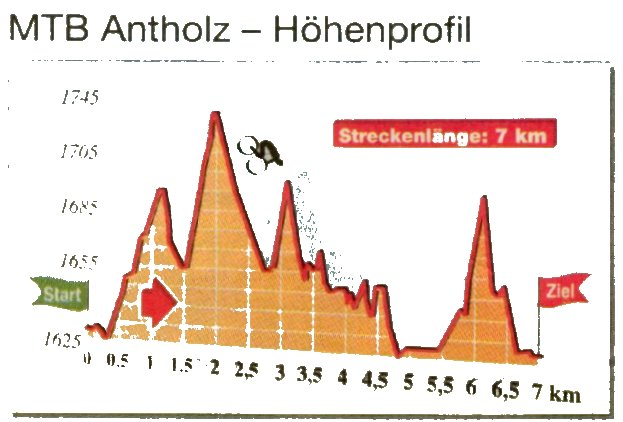
\includegraphics[width=6.5cm]{2te/funktion/bilder/antholz.jpg}
\end{minipage}
\begin{minipage}{7cm}
\bn \item Was wird in der nebenstehenden Graphik zugeordnet? Handelt es sich um eine Funktion?
\item Bestimme die Definitions- und Wertemenge! \en
\end{minipage}

\item Kennst du das Morsealphabet? Handelt es sich dabei um eine Funktion?

\end{enumerate}
\ea




\section{Funktionsgleichung und Funktionswert}

Die Einf\"{u}hrungsbeispiele aus dem vorhergehenden Kapitel stammen zum Teil nicht aus der Mathematik. Sie
sollten aber einen ersten Einblick in diese Materie verschaffen und aufzeigen, dass Funktionen, also
Zuordnungen, uns wirklich \"{u}berall begegnen k\"{o}nnen (wenn wir sie nur erkennen - wollen).

\ba
Versuche selbst eine Funktion aus dem Alltag anzugeben.
\ea

Wir werden uns nun etwas einschr\"{a}nken und uns auf Zahlenbeispiele
konzentrieren. So werden nun f\"{u}r die Definitons- und Wertemenge
meistens Zahlenmengen (z.B. $\mathbb{N, Z, Q, R, R_+} \dots$)
stehen. Wollen wir alle Zahlen zulassen, so wird es sich oft um
Funktionen handeln mit $D= \dots$ und  $W= \dots$, also eine
Zuordnung der Art: $f: \mathbb{R} \mapsto \mathbb{R}$.

Dann ist es aber auch nicht notwendig, jedes Mal diese Mengen eigens anzugeben. So schreiben wir dann z.B.
f\"{u}r die Funktion
\[\begin{array}{rrcl}
  f: & \mathbb{R} & \rightarrow & \mathbb{R} \\
   & x & \mapsto & x^2-1
\end{array}\]
nur mehr die sog. Funktionsgleichung $f(x)=x^2-1$ oder $y=x^2-1$. Dies bedeutet, dass $y$ gleich $f(x)$
(lies: "`f von x"') zu sehen ist. Genauer:

\bd \label{9}
Jede beliebige Funktion
\[\begin{array}{rrcl}
  f: & \mathbb{R} & \rightarrow & \mathbb{R} \\
   & x & \mapsto & y
\end{array}\] besitzt eine {\bf Funktionsgleichung}, n\"{a}mlich
y=f(x). Dabei handelt es sich um eine Gleichung mit zwei
Variablen.
\ed

\bb\label{2.1}
Wie lautet die Funktionsgleichung zur Funktion:
\[\begin{array}{rrcl}
  f: & \mathbb{R} & \rightarrow & \mathbb{R} \\
   & x & \mapsto & -\frac{x}{3}?
\end{array}\]
Wieviele L\"{o}sungen hat diese Gleichung? Gib zwei L\"{o}sungen an.
\eb

\bd
Wenn $f$ eine Funktion ist, so versteht man unter dem {\bf Funktionswert} von $x$, kurz $f(x)$ (lies: "`f von x"'),
jene Zahl, die durch die Funktion $f$ der Zahl $x$ zugeordnet wird.
\ed

\bb
Gegeben ist die Funktion: $f(x)=x^2-2x$. Berechne die
Funktionswert $f(2)$ und $f(-\frac{2}{3})$.
\eb

\ba \label{5}  \label{2.2}
\begin{enumerate}
\item Was ist eine Funktion?
\item Bestimme die Funktionswerte $f(0)$ und $f(\frac{1}{2})$ f\"{u}r
die Funktion $f(x)=4x^2-2x+1$.
\item Bestimme die Funktionsgleichung zur Funktion
\[\begin{array}{rrcl}
  f: & \mathbb{R} & \rightarrow & \mathbb{R} \\
   & x & \mapsto & \frac{7x-3}{2}
\end{array}\] und berechne $\frac{5}{7}$.

\item Gegeben ist die Funktion, die jeder Seitenl\"{a}nge den Umfang
des Quadrates zuordnet. Gib dazu die Funktion samt Definitions-
und Wertemenge und die Funktionsgleichung an. Berechne einige
Funktionswerte, indem du die folgende Tabelle ausf\"{u}llst:
\[\begin{array}{|c|c|c|c|c|c|}
\hline
  x & 1 & 2 & 8 & 10 & -4 \\ \hline
  f(x) &  &  &  &  & \\ \hline
\end{array}\]
\end{enumerate}
\ea



\section{Der Graph der Funktion und die Nullstellen}


\bb {\tiny .}

\begin{minipage}{8cm}
Funktionsgraphen begegnen uns sehr h\"{a}ufig immer und \"{u}berall - beispielsweise in den Medien, in Schulb\"{u}chern
anderer F\"{a}cher (!) und vielerorts mehr.

Nur oft werden die entsprechenden Graphiken nicht mit dem Begriff der Funktion in Verbindung gebracht, oder
auch nur (um etwa den Leser und Betrachter nicht abzuschrecken) nicht erw\"{a}hnt.

Hier ein Beispiel einer typischen Anwendung des Funktionsgraphen zur Veranschaulichung eines komplizierten
Sachverhaltes.

\end{minipage}
\begin{minipage}{6cm}
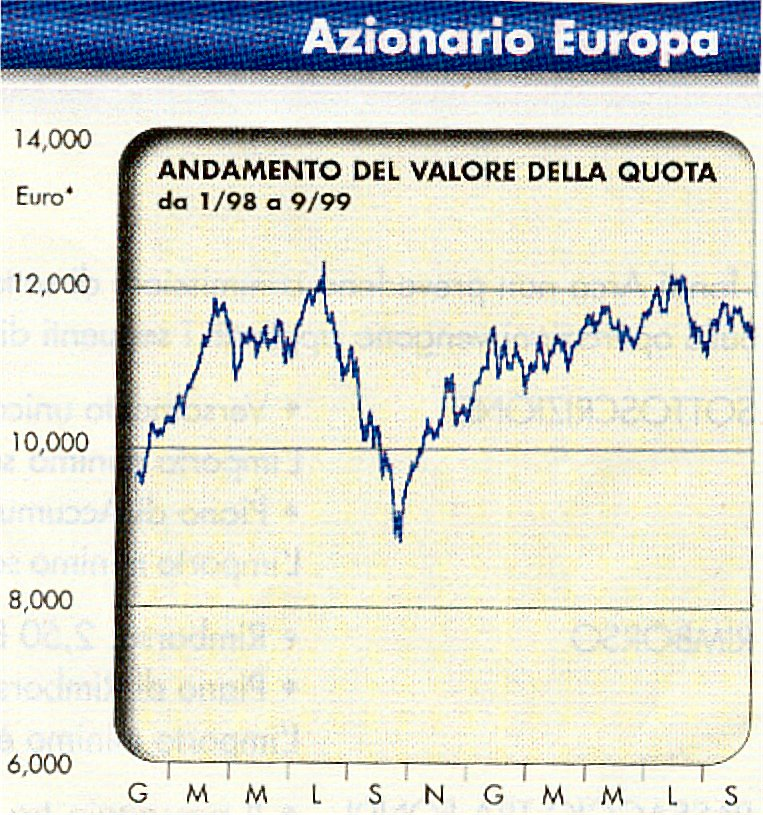
\includegraphics[width=5cm]{2te/funktion/bilder/fkt_aktien.jpg}
\end{minipage}

\eb


Haben wir eine mathematische Funktion, also eine Funktion von $f: \mathbb{R} \rightarrow \mathbb{R}$,
gegeben, so wird jeder (reellen) Zahl $x$ eine Zahl $y$ zugeordnet. Daraus ergeben sich Zahlenpaare $(x;y)$,
die in ein (kartesisches\footnote{nach R.~Descartes, genannt Cartesius, 1596 bis 1650. Die Besonderheit
dieses Koordinatensystems ist, das die Achsen zueinander rechtwinklig sind.}) Koordinatensystem eingezeichnet
werden k\"{o}nnen. So erh\"{a}lt man eine graphische Darstellung einer Funktion - den Graphen der Funktion. Genauer:

\bd
Unter dem {\bf Graph der Funktion} $f$ versteht man die Menge aller Zahlenpaare $(x;f(x))$.
\ed

\begin{Bem}{\bf Praktische Konstruktion des Graphen:}
\begin{enumerate}
\item Man stellt eine Wertetabelle auf, indem man f\"{u}r gen\"{u}gend viele,
geeignet gew\"{a}hlte Zahlen den Funktionswert berechnet. Tip: die Zahl $0$ sollte in der Regel immer gew\"{a}hlt
werden, da die Berechnung des Funktionswerte oft sehr einfach ist. (Was man unter "`gen\"{u}gend viele"' und
"`geeignet gew\"{a}hlte"' Zahlen versteht, h\"{a}ngt von der gegebenen Funktion ab; einige Erfahrung ist sicherlich
daf\"{u}r notwendig.)
\item Man zeichnet diese Zahlenpaare in einem Koordinatensystem
ein und verbindet sie durch eine Kurve (oder Geraden). Dabei
k\"{o}nnen die Einheiten auf der x- und y-Achse beliebig und
verschieden (!) geeignet gew\"{a}hlt werden.
 \end{enumerate}
\end{Bem}

\bb
 Zeichne die Funktionsgraphen der folgenden Funktionen:
\label{6}\label{2.3}\label{2.4}
\begin{enumerate}
\item $f(x)=\frac{1}{2}x$
\item $f(x)=-2x+1$
\item $f(x)=x^2-1$
\end{enumerate}
\eb

\ba Zeichne die Funktionsgraphen der folgenden Funktionen:
\label{8}\label{2.5}
\begin{enumerate}
\item $f(x)=-x$
\item $f(x)=|x|$ (Betragsfunktion, vgl. p. \pageref{7})
\item $f(x)=-x^2+4$
\end{enumerate}


\item Welche Darstellungen geh�ren zu einer Funktion?

%\begin{center}
%\includegraphics[width=7cm]{scanimage200501.jpg}
%\end{center}


\ea

\begin{Bem}
\begin{enumerate}
\item Die eingezeichneten Punkte d\"{u}rfen nur dann verbunden werden,
wenn $D=\mathbb{R}$ ist. Handelt es sich z.B. um eine Zuordnung
zwischen Personen und Eintrittsgeld bei einem Theaterbesuch, so
hat ein Verbinden der Punkte keinen Sinn; warum?
\item Der Funktionsgraph ist sehr sehr n\"{u}tzlich. Oft, vor allem im
Alltag, z.B. in Zeitschriten, in Lehrb\"{u}chern usw. wird auf die
Angabe der Funktion verzichtet und nur der Funktionsgraph
dargestellt. Weiters dient er:
\begin{enumerate}
\item zur Veranschaulichung der Funktion
\item zur graphischen Bestimmung von Funktionswerten (x gegeben, y
gesucht)
\item zur graphischen Bestimmung der Werte x, die durch die
Funktion einem bestimmten $y$ zugeordnet werden ($x$ gesucht, $y$
gegeben).
\item zur graphischen Bestimmung der Schnittpunkte des
Funktionsgraphen mit der x-Achse; dies f\"{u}hrt zur folgenden
Definition:
\end{enumerate}
\end{enumerate}
\end{Bem}

\bd
Gegeben ist eine Funktion $f$. Ein $x \in D$ bezeichnet man als
{\bf Nullstelle}, falls $f(x)=0$ gilt.
\ed

Man sucht also die Werte aus der Definitionsmenge die den
Funktionswert $0$ ergeben. Dies sind dann eben genau die
Schnittpunkte des Funktionsgraphen mit der x-Achse.

\bb
\begin{enumerate}
\item  Ermittle graphisch $f(-2)$ und $f(4)$ von Bsp. \ref{6} Nr. 2.
Bestimme weiters die Nullstellen. Kontrolliere deine Ergebnisse
rechnerisch.
\item Ermittle graphisch alle $x$, f\"{u}r die $y=9$ bzw. $y=2$ ist
aus Bsp. \ref{6} Nr. 3. Gibt es Nullstellen? Kontrolliere wieder
deine Ergebnisse rechnerisch.
\end{enumerate}
\eb




\ba
Diese Aufgabe bezieht sich auf die 3 Funktionen aus Aufgabe
\ref{8} Nr.1, 2 und 3:
\begin{enumerate}
\item Zeichne die 3 Graphen indem du dir gen\"{u}gend Funktionswerte berechnest.
\item Bestimme jeweils $f(1)$ graphisch und kontrolliere rechnerisch.
\item Bestimme (ungef\"{a}hr) alle $x$, so dass $f(x)=8$ gilt.
\"{U}berpr\"{u}fe dein Ergebnis rechnerisch.
\item Bestimme die Nullstellen zeichnerisch und rechnerisch.
\end{enumerate}
\ea

\begin{Bem}{\bf Zusammenhang: Graph und Funktionsgleichung}
Wie in Definition \ref{9} auf Seite \pageref{9} erw\"{a}hnt, handelt
es sich bei der Funktionsgleichung um eine Gleichung mit zwei
Variablen. Eine Gleichung dieser Art hat unendlich viele L\"{o}sungen,
denn man kann sich einfach f\"{u}r eine Variable eine Zahl w\"{a}hlen und
die andere berechnen.

Andererseits kann eine Funktionsgleichung dazu verwendet werden um
Zahlenpaare zu berechnen, die, eingezeichnet in ein
Koordinatensystem, den Funktionsgraphen ergeben.

Zusammenhang: der Funktionsgraph besteht aus den L\"{o}sungen der
Funktionsgleichung oder umgekehrt:

jede L\"{o}sung der Funktionsgleichung, also jedes Zahlenpaar, das die
Funktionsgleichung erf\"{u}llt, liegt auf dem Graphen der Funktion.
\end{Bem}

\bn \item 
Gegeben ist die Funktion $f(x)=-x+5$. \label{2.6} \"{U}berpr\"{u}fe
 zeichnerisch und  rechnerisch
ob die Punkte $(0;0)$, $(-\frac{7}{2};8,5)$ und $(4;2)$ auf dem Funktionsgraphen liegen und somit L\"{o}sungen
der Funktionsgleichung sind.
\item 
 Liegen die Punkte $(3;9)$ und $(-2;-4)$ auf dem Graphen der Funktion $f(x)=x^2$?  Begr\"{u}nde zeichnerisch und  rechnerisch! Berechne auch die  Nullstellen dieser Funktion! 
\en



\section{Umkehrfunktionen}

\subsection{Allgemeine Definition und Beispiele}
 \bd  Die Funktion $f: D \rightarrow W$ mit $D, W \subseteq \mathbb{R}$ hei{\ss}t {\it bijektiv} oder {\it
umkehrbar}, wenn gilt: \bn \item F\"{u}r alle $x_1, x_2 \in D$ mit $x_1 \neq x_2$ gilt: $f(x_1)\neq f(x_2)$;
\item f\"{u}r jedes $y \in W$ gibt es ein $x \in D$ mit $f(x)=y$.\en  \ed  

\ba \bn \item Gib eine Beispiel f\"{u}r eine umkehrbare (bijektive) Funktion an. \item Finde zwei Beispiele von
Funktionen, welche nicht umkehrbar sind, wobei beim ersten Beispiel die erste Bedingung und beim zweiten
Beispiel die 2. Bedingung nicht erf\"{u}llt ist. Visualisiere den Sachverhalt mit Hilfe von einem Pfeildiagramm
(2 Mengen und die Zuordnung zeichnen). \en \ea  

\bd  Ist $f$ umkehrbar, dann ist durch $$f^{-1}(y)=x
:\Leftrightarrow f(x)=y$$ eine Funktion $f^{-1}:D \rightarrow W$ definiert, welche als {\bf Umkehrfunktion}
oder auch {\it inverse Funktion} von $f$ bezeichnet wird. \ed  

\begin{Bem}
Per Definition gilt: $f^{-1}(f(x))=x \qquad \mbox{f\"{u}r alle} \quad x \in D \qquad \mbox{und} \qquad
f(f^{-1}(x))=x \qquad \mbox{f\"{u}r alle} \quad x \in D$
\end{Bem}

Es gibt auch unendlich viele Funktionen, die keine Umkehrfunktion besitzen. Schr\"{a}nkt man aber die
Definitionsmenge ein, so kann man eine Umkehrfunktion angeben.

\bb Die Funktion $y=x^4$ ist auf $D=\mathbb{R}$ nicht umkehrbar. Nimmt man aber $D=\mathbb{R}^+$ so ist die
Funktion streng monoton und deshalb umkehrbar.\eb



\bs  \label{dfdf} Die Graphen von $f$ und $f^{-1}$ im kartesischen Koordinatensystem sind {\it symmetrisch}
bez\"{u}glich der ersten Winkelhalbierenden $y=x$. \es 

Damit bekommen wir auch eine Anleitung zum Auffinden einer Umkehrfunktion:

Ist $f$ umkehrbar, so gewinnt man die Funktionsgleichung von $f^{-1}$ durch (formales) Vertauschen der
Variablen in $y=f(x)$ und Aufl\"{o}sen nach $y$: $$y=f(x) \qquad \Rightarrow \qquad x=f(y)   \qquad  \Rightarrow \qquad f^{-1}(x)=y$$

\ba \bn \item Finde die Umkehrfunktion zu $f(x)=-\frac12x+3$ und zeichne beide Funktionsgrafen in das gleiche
Koordinatensystem ein. \"{U}berpr\"{u}fe anschlie{\ss}end Satz \ref{dfdf} (Seite \pageref{dfdf}).
\item Gegeben sei die Funktion $f(x)=\sqrt{x}$ und der Definitionsbereich $\{9,16,25,36\}$.     Bestimme den
Wertebereich der Funktion. Bestimme ihre Umkehrfunktion. Bestimme Definitionsbereich und Wertebereich der Umkehrfunktion.
\en
\ea

\bme 
{\bf �ber die Umkehrung einer Funktion}
\bn \item
Jede {\it streng monoton wachsende} oder {\it fallende} Funktion ist {\it umkehrbar}
\item Bei der Umkehrung einer Funktion werden Definitions- und Wertemenge miteinander vertauscht.
\item Die Umkehrfunktion $g$ einer Funktion $y=f(x)$ findet man  (oft aber nicht immer) indem man  \bn \item  $y$ und $x$ vertaucht \item und nach $y$ wieder die Gleichung aufl�st.\en 
\item Zeichnerisch erh�lt man das Schaubild der Umkehrfunktion durch {\it Spiegelung} des Funktionsgraphen an der 1. Winkelhalbierenden (Gerade: $y=x$)
 
\en 
\eme 



\subsection*{\"{U}bungen zur Schularbeit}
\ba
\begin{enumerate}
\item $g$ ist die Funktion, die jeder rationalen Zahl ihr Quadrat
zuordnet. \bn \item Dann gilt: \[\begin{array}{ccccc}
  g(2)=\dots & g(0)=\dots & g(4)=\dots & g(\frac{1}{2})=\dots & g(0,4)=\dots \\
  g(3)=\dots & g(1)=\dots & g(-4)=\dots & g(-\frac{1}{3})=\dots & g(-0,5)=\dots
\end{array}\]
\item Zeichne mit diesen berechneten Werten den Funktionsgraph.
\item Wie lautet die Funktionsgleichung?
\item Wie m\"{u}ssen Definitionsmenge und/oder Wertemenge ver\"{a}ndert werden, damit eine Umkehrfunktion existiert?
Wie lautet ihre Funktionsgleichung? \en

\item Erg\"{a}nze:

{\it Eine Funktion $f$ ist eine $\dots$. Sie ordnet jeder Zahl $x$
ihrer $\dots$ wieder eine Zahl zu, den. sog. $\dots$ von $x$
(Bezeichnung: $\dots$).

Zwischen $f$ und $f(x)$ besteht der folgende Unterschied: $f$
bezeichnet die $\dots$, dagegen ist $f(x)$ eine $\dots$.}

\item Die Funktion $g$ ist definiert durch $g(x)=x^2+2x$.
\begin{enumerate}
\item Die Funktion $g$ hat die Definitionsmenge $D=\dots$.
\item Berechne $g(3)$, $g(\frac{5}{2})$, $g(-3)$ und $g(1)$!
\item Gib an: $g(z)=\dots$, $g(u)=\dots$.
\item Welche Zahlen haben den Funktionswert $8$?
\item Gibt es Nullstellen?

\end{enumerate}

\item Wir betrachten die Funktion
\[\begin{array}{rrcl}
  h:  & u & \mapsto & \frac{u}{u^2-4}
\end{array}\]
Welchen Definitionsbereich hat $h$? Berechne $h(1)$, $h(10)$,
$h(-\frac{3}{2})$ und $h(2)$.
\item
\begin{enumerate}
\item Zeichne den Graphen von $g(x)=0,6\cdot x+1$.
\item Um was f\"{u}r eine Kurve handelt es sich offensichtlich?
\item Wie viele Punkte h\"{a}tten also f\"{u}r das Zeichnen des Graphen
gen\"{u}gt? \item Berechne die Nullstellen! \item Bestimme die Funktionsgleichung der Umkehrfunktion.
\end{enumerate}
\item
\begin{enumerate}
\item Erg\"{a}nze:

{\it Unter einer L\"{o}sung der Gleichung \[y=2-\frac{1}{5}x^2\]
versteht man ein $\dots$, das beim Einsetzen in die Gleichung
diese $\dots$.}

\item Versuche so eine L\"{o}sung anzugeben.

\item Liegen die Punkte $P=(-4,5;-2)$ und $Q=(-1,5;1,6)$ auf dem
Graphen dieser Funktion? \end{enumerate}
\item Kann die Kurve aus der Abbildung  der Graph einer Funktion
sein? Warum nicht?

\input{2te/funktion/bilder/fkt1.pic}

\item Kann eine horizontale Gerade der Graph einer Funktion sein?

Kann eine vertikale Gerade der Graph einer Funktion sein?
\end{enumerate}

\ea


